% Supplementary Figure S2 - sequence generation mechanism.
% Source of truth for the caption: ../mechanism_figure/fig_s2_caption.md
% Graphic: ../mechanism_figure/fig_s2.pdf  (vector, cropped to content,
% 180.6 x 184.5 mm; BMC scales full-width figures to 170 mm, giving 173.7 mm
% of height and leaving ~24 mm of the 225 mm figure+legend cap for the legend).
% Requires: graphicx
\begin{figure}[p]
\centering
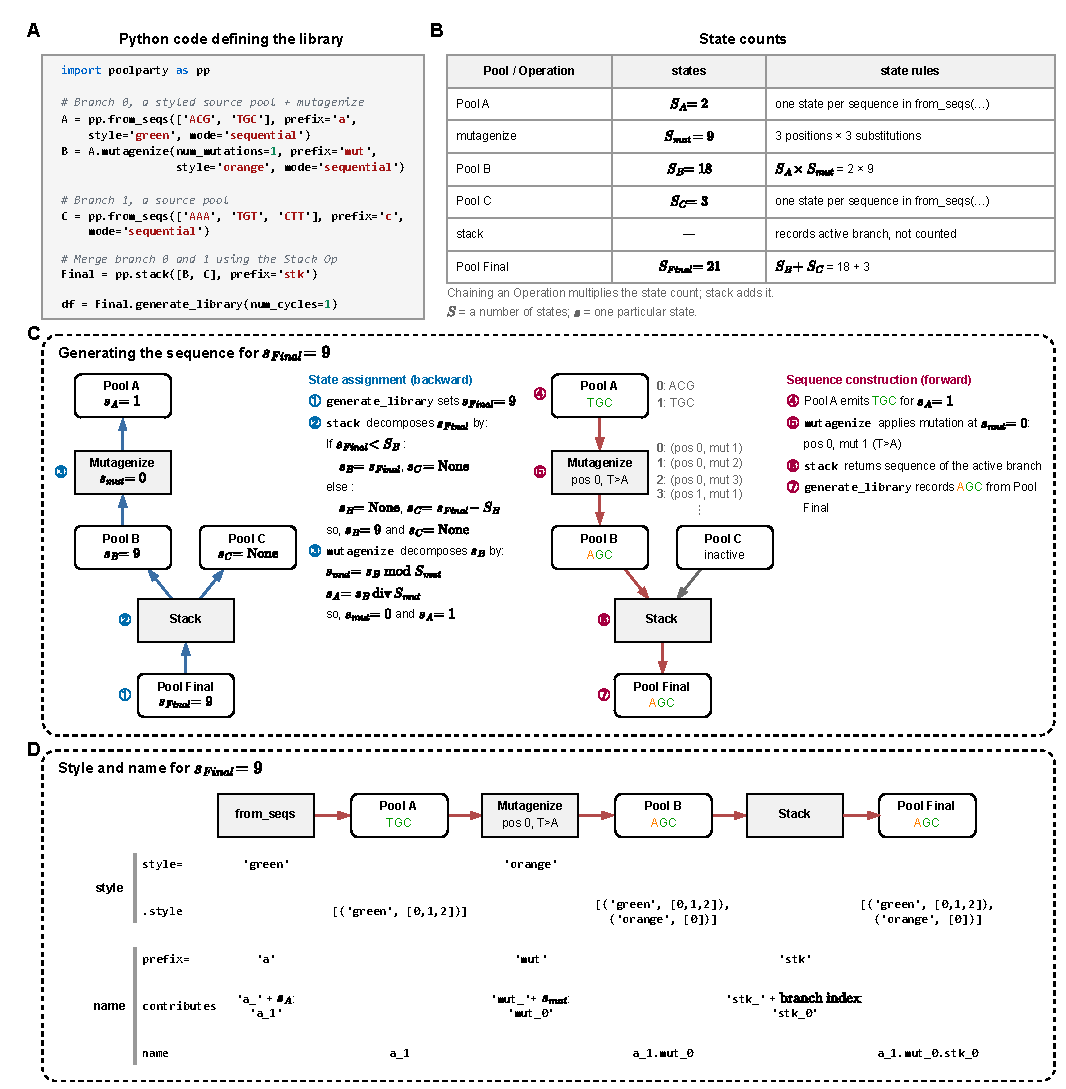
\includegraphics[width=\textwidth]{../mechanism_figure/fig_s2}
\caption{\textbf{A worked example of sequence generation.}
\textbf{(A)} Python code defining the library.
\textbf{(B)} Number of states of each Pool and Operation.
\textbf{(C)} Generating the sequence for $s_{Final} = 9$. Left: state assignment (blue).
Right: sequence construction (magenta). Lists beside Pool A and \texttt{mutagenize} show
which sequence or mutation each state selects. Inactive branches are shown in grey.
\textbf{(D)} Style and name for the same sequence. Sequences are carried through the DAG as
\texttt{Seq} objects, which hold the sequence string together with its \texttt{.style}. The
\texttt{style} and \texttt{prefix} arguments are supplied to Operations; the resulting
\texttt{.style} and name are held by Pools. Sequence characters are colored by their
\texttt{.style} entries; where entries overlap, the last one applies.}
\label{fig:figureS2}
\end{figure}
